% CS224R Final Project Poster
% Stanford Gemini theme, 36"x24" landscape (recommended dimensions)
% Compile with XeLaTeX

\documentclass[final]{beamer}

% ====================
% Packages
% ====================

\usepackage[T1]{fontenc}
\usepackage{lmodern}
% 36" x 24" = 91.44 cm x 60.96 cm (rounded to 91 x 61 cm)
\usepackage[size=custom,width=91,height=61,scale=1.0]{beamerposter}
\usetheme{gemini}
\usecolortheme{stanford}
\usepackage{graphicx}
\usepackage{booktabs}
\usepackage{tikz}
\usepackage{pgfplots}
\pgfplotsset{compat=1.17}

\graphicspath{{plots/}}

% ====================
% Lengths — 3 columns
% ====================

\newlength{\sepwidth}
\newlength{\colwidth}
\setlength{\sepwidth}{0.025\paperwidth}
\setlength{\colwidth}{0.3\paperwidth}

\newcommand{\separatorcolumn}{\begin{column}{\sepwidth}\end{column}}

% ====================
% Header / metadata
% ====================

\title{Offline RL for Adaptive Vocabulary Selection \\
       in Conversational Language Tutoring}

\author{Onyinyechi Okoye}

\institute[shortinst]{Computer Science, Stanford University \quad CS224R Spring 2026}

\footercontent{
  Code: \href{https://github.com/onyieo/adaptive-vocab-rl}{github.com/onyieo/adaptive-vocab-rl} \hfill
  CS224R Final Project \hfill
  \href{mailto:onyie@stanford.edu}{onyie@stanford.edu}}

\begin{document}

% Stanford logo top-right
\addtobeamertemplate{headline}{}{
    \begin{tikzpicture}[remember picture,overlay]
      \node [anchor=north east, inner sep=2cm]
            at ([xshift=0.0cm,yshift=1.5cm]current page.north east)
      {\includegraphics[height=5.0cm]{stanford_logos/Block_S_2_color.png}};
    \end{tikzpicture}
}

\begin{frame}[t]
\begin{columns}[t]
\separatorcolumn

% =====================================================================
% COLUMN 1 — Q1 Problem, Q2 Why It Matters, Q3 Prior Work
% =====================================================================
\begin{column}{\colwidth}

  \begin{block}{1. What is the problem?}
    A conversational language tutor must decide at every turn:
    \emph{which vocabulary should the tutor's response target?} Each turn
    presents a mix of words the learner has never seen, words being
    acquired, and words due for review. This is a sequential decision
    problem with delayed, multi-objective rewards: the effect of
    introducing a word now on long-term retention is not observed until
    future sessions.
  \end{block}

  \begin{block}{2. Why is it interesting and important?}
    The choice involves a genuine multi-way trade-off:
    \begin{itemize}
      \item \textbf{Long-term retention} — words must come back before they decay
      \item \textbf{Curriculum pacing} — too many new words at once overwhelms the learner
      \item \textbf{Conversational naturalness} — the tutor's response must still
            sound like dialogue, not a flashcard drill
    \end{itemize}
    A real product (Duolingo, Anki, LingoChamp, etc.) ships some hand-coded
    spaced-repetition rule. A principled RL approach has the potential to
    discover scheduling strategies no fixed heuristic can match.
  \end{block}

  \begin{block}{3. Why hasn't it been solved before?}
    \textbf{Spaced repetition (FSRS, SM-2)} \cite{fsrs} schedules
    flashcards in isolation — no mechanism for embedding review in
    natural conversation, no joint reasoning about introducing new vocabulary.

    \textbf{RLHF-style methods} \cite{rlhf} treat the LLM as the policy and
    can't reason about long-horizon retention; the LLM optimizes a
    naturalness reward turn-by-turn.

    \textbf{Educational RL} \cite{rafferty} works on isolated problems
    (which exercise to assign), never on item selection mediated through a
    generative LLM producing free-form dialogue.

    \textbf{Our contribution}: a \emph{hierarchical control} framing where
    RL operates over latent linguistic constraints and a frozen LLM
    realizes them as natural conversation.
  \end{block}

  \begin{block}{4. Key components of our approach}
    \begin{center}
      \begin{tikzpicture}[
          node distance=0.6cm and 0.7cm,
          box/.style={rectangle, draw=stanfordred, very thick, rounded corners,
                     minimum height=1.4cm, minimum width=3.2cm, align=center,
                     text width=3.0cm, font=\footnotesize},
          smallbox/.style={rectangle, draw=black!50, thick, rounded corners,
                     minimum height=1.1cm, minimum width=2.4cm, align=center,
                     text width=2.2cm, font=\scriptsize},
          arrow/.style={->, very thick, stanfordred, >=latex}]
        \node[box] (policy) {Offline RL Policy $\pi(a|s)$ \\ (IQL / CQL)};
        \node[smallbox, right=of policy] (action) {Action: directive\\$(n_{\text{new}}, n_{\text{act}}, n_{\text{rev}})$};
        \node[smallbox, right=of action] (llm) {Frozen LLM\\(Claude Sonnet)};
        \node[smallbox, below=of llm] (utter) {Japanese\\conversational turn};
        \node[smallbox, below=of action] (sim) {Student\\simulator\\(FSRS)};
        \node[smallbox, below=of policy] (state) {State $s$:\\per-word stats};
        \draw[arrow] (policy) -- (action);
        \draw[arrow] (action) -- (llm);
        \draw[arrow] (llm) -- (utter);
        \draw[arrow] (utter) -- (sim);
        \draw[arrow] (sim) -- (state);
        \draw[arrow] (state) -- (policy);
      \end{tikzpicture}
    \end{center}
    \begin{itemize}
      \item \textbf{State} $s_t$: per-word stability, retrievability, difficulty,
            usage counts; session position. 500 JLPT N5/N4/N3 words.
      \item \textbf{Action} $a_t$: structured directive
            $(n_{\text{new}}, n_{\text{active}}, n_{\text{review}})$
            summing to 5 words (21 discrete actions).
      \item \textbf{Reward} $r_t$: see Findings (the headline result).
      \item \textbf{Methods}: IQL \cite{iql}, CQL \cite{cql} (offline);
            PPO \cite{ppo} (online upper bound); Random, FSRS, FSRS+New,
            RuleBased, SmartFSRS (heuristics).
    \end{itemize}
  \end{block}

\end{column}

\separatorcolumn

% =====================================================================
% COLUMN 2 — Q5 Findings (reward design + headline)
% =====================================================================
\begin{column}{\colwidth}

  \begin{alertblock}{5. Key findings — Reward design $\gg$ algorithm choice}
    Same algorithms, two rewards, \textbf{6$\times$ retention improvement}
    across every RL method from the reward redesign alone.

    \heading{v3 reward}
    $$r_t = \underbrace{\Delta R_{\text{total}}/N}_{\text{coverage}}
            \;-\; \underbrace{\alpha \cdot \max(0, n_{\text{new}} - 1)^2}_{\text{naturalness penalty}}
            \;+\; \underbrace{\lambda \cdot \tfrac{\#\{R{>}0.5\}}{N}}_{\text{session-end retention bonus}}$$

    The naturalness penalty stops policies from cramming many new words
    into one turn; the session-end bonus directly rewards what the
    proposal calls the actual goal.
    \vspace{0.3cm}
    \begin{figure}
      \centering
      
\includegraphics[width=0.95\colwidth]{reward_design_impact.png}
    \end{figure}
  \end{alertblock}

  \begin{block}{Final retention numbers}
    \begin{figure}
      \centering
      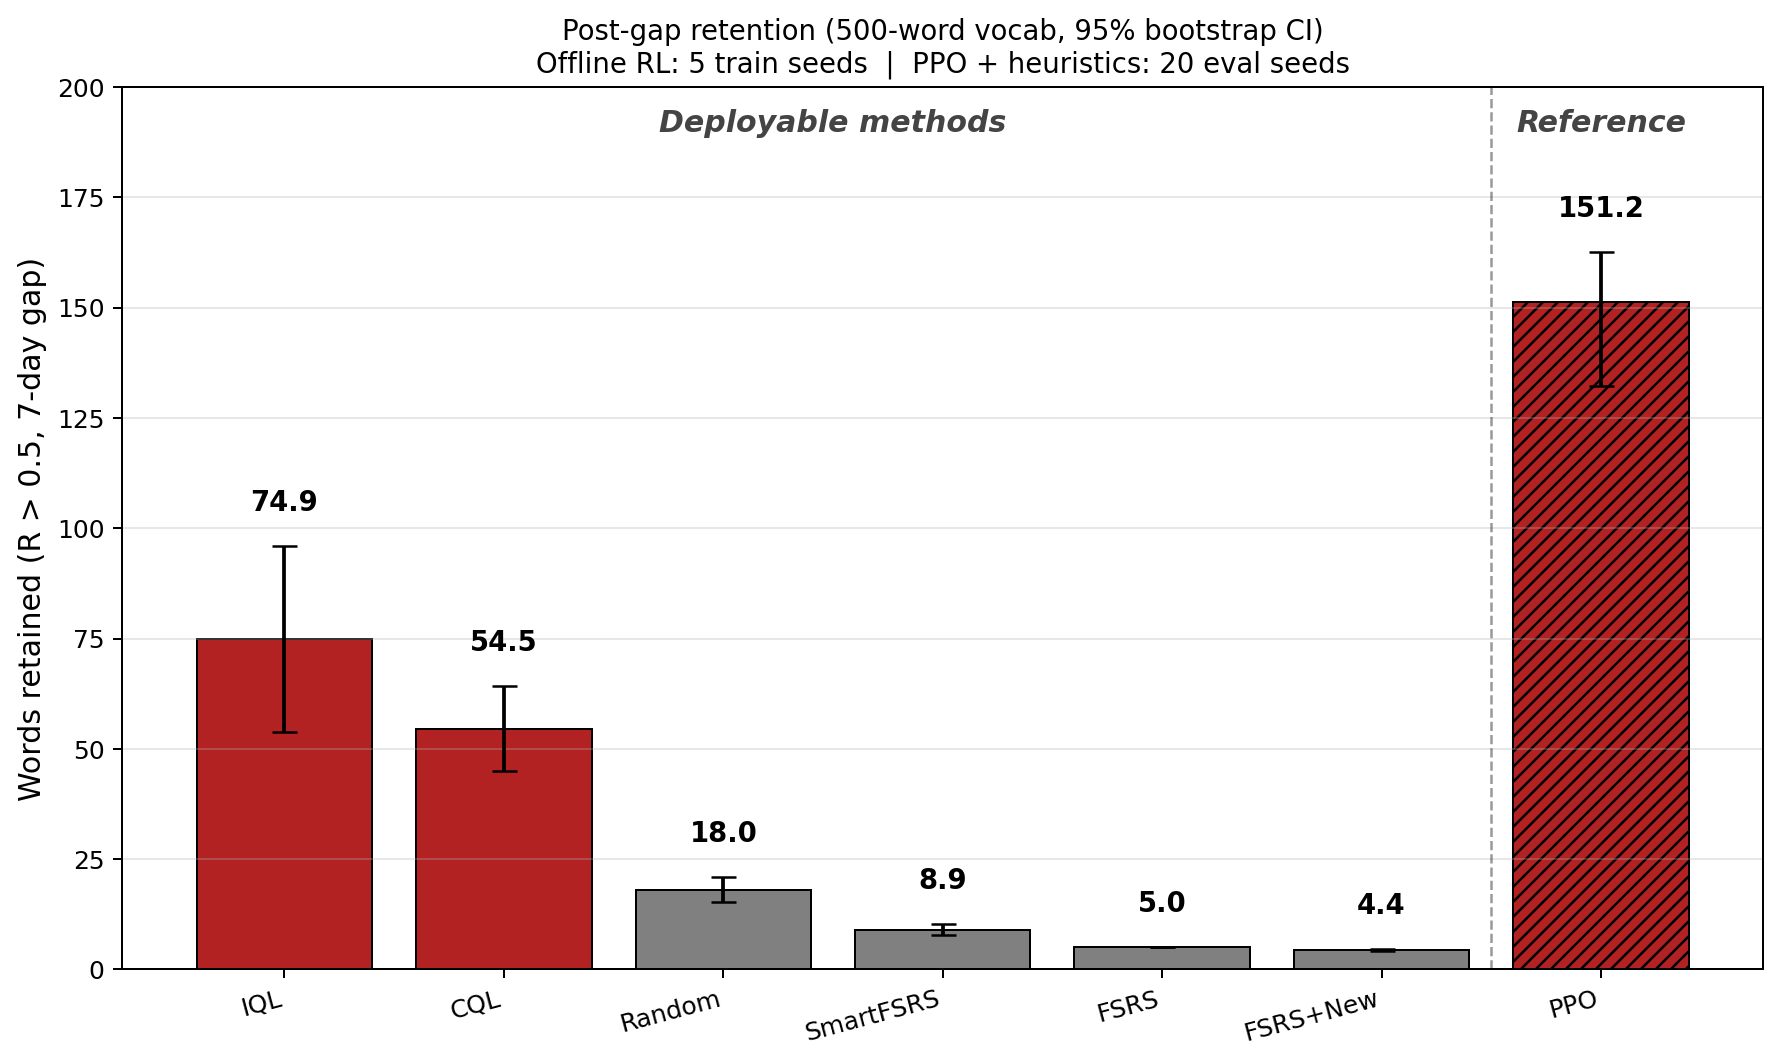
\includegraphics[width=0.98\colwidth]{headline_retention_20seeds.png}
    \end{figure}
    500 words, 20 eval seeds, 95\% bootstrap CIs. \textbf{Every RL method
    beats every heuristic by 5--30$\times$.} Online RL (PPO) exceeds
    offline RL by $\sim$1.8$\times$ — the cost of the deployment-realistic
    offline constraint (in production you cannot expose real students to a
    learning policy).
  \end{block}

\end{column}

\separatorcolumn

% =====================================================================
% COLUMN 3 — Q5 (more findings) + Q6 + Q7
% =====================================================================
\begin{column}{\colwidth}

  \begin{block}{Adaptive pacing emerges from training}
    \begin{figure}
      \centering
      
\includegraphics[width=0.98\colwidth]{action_distribution_v3.png}
    \end{figure}
    Action mix by turn-in-session. RL methods (right panels) learn
    intra-session pacing: heavy on new-word actions early, shift to review
    late. \emph{No hand-coded baseline shows this structure.}
  \end{block}

  \begin{block}{Retention vs naturalness Pareto frontier}
    \begin{figure}
      \centering
      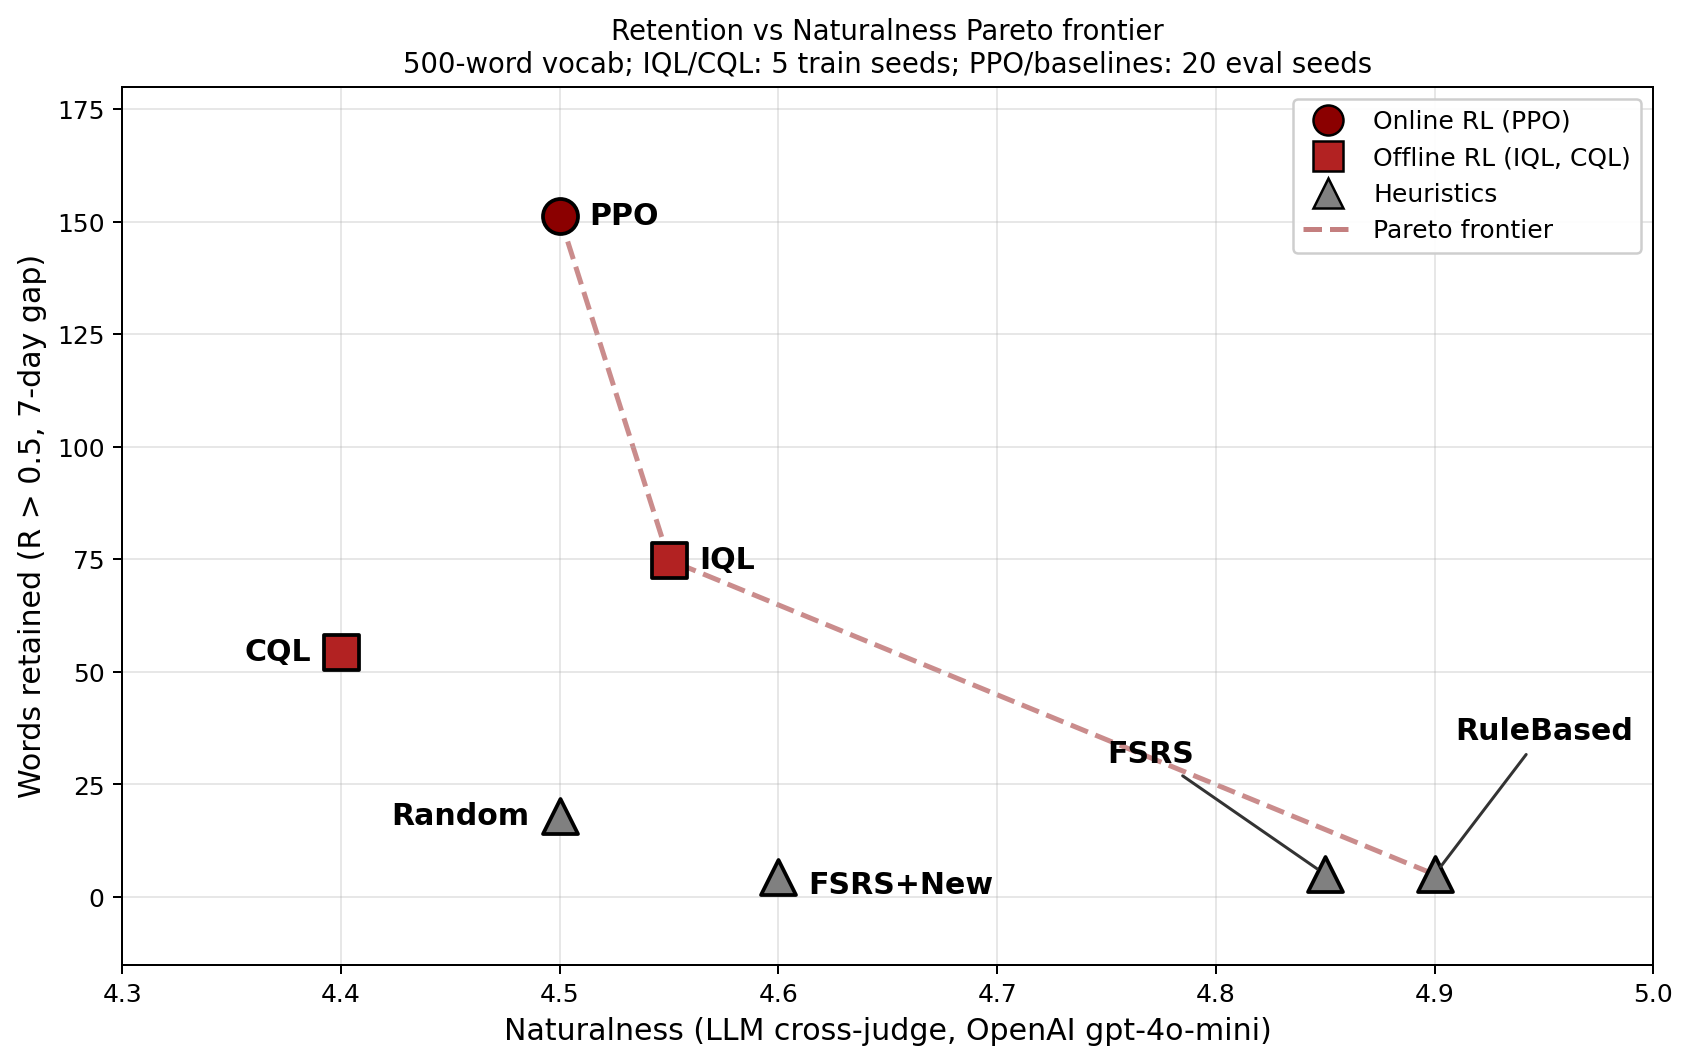
\includegraphics[width=0.98\colwidth]{pareto_retention_naturalness.png}
    \end{figure}
    Naturalness judged by \emph{cross-family} OpenAI gpt-4o-mini (the tutor
    is Claude Sonnet — eliminates self-preference bias). PPO matches Random
    on naturalness but at \emph{8$\times$ the retention}; offline IQL has
    higher naturalness than PPO at 56\% of retention.
  \end{block}

  \begin{block}{6. Takeaways and limitations}
    \heading{What audiences can learn}
    \begin{itemize}
      \item \textbf{Reward design dominates algorithm choice} for this domain
      \item \textbf{Coverage metrics mislead}: Random scored 81 acquired but
            only 18 retained after 7 days. Stickiness matters.
      \item \textbf{Hierarchical RL/LLM control} works: structured directives
            are tractable as RL actions; the LLM handles naturalness via prompting
    \end{itemize}
    \heading{Honest limitations}
    \begin{itemize}
      \item Simulator dynamics are hand-tuned; no human pilot yet
      \item Action space is coarse (21 directives); finer-grained word
            selection is future work
      \item Wide CIs on offline RL (e.g.\ IQL: [52.6, 119.0])
            indicate seed sensitivity
    \end{itemize}
  \end{block}

  \begin{block}{7. Planned before final report}
    \begin{itemize}
      \item \textbf{Tighter CIs}: multi-seed training of IQL/CQL on Modal
      \item \textbf{BC-of-PPO ablation}: does offline RL exceed simple imitation?
      \item \textbf{Top-$k$ action space}: per-word selection beyond the 21-action directive
      \item \textbf{Extended OOD robustness}: forgetting rate, difficulty distribution, combined OOD held-out sims
    \end{itemize}
  \end{block}

  \begin{block}{References}
    \nocite{*}
    \footnotesize{\bibliographystyle{plain}\bibliography{poster}}
  \end{block}

\end{column}

\separatorcolumn
\end{columns}
\end{frame}

\end{document}
